%\documentclass[ignorenonframetext, compress, 9pt, xcolor=svgnames]{beamer} 
\documentclass[notes, ignorenonframetext, compress, 10pt, xcolor=svgnames, aspectratio=169]{beamer} 
%\documentclass[notes, ignorenonframetext, compress, 10pt, xcolor=svgnames, aspectratio=169]{beamer} 
\usepackage{pgfpages}
\usepackage{pdfpages}
% These slides also contain speaker notes. You can print just the slides,
% just the notes, or both, depending on the setting below. Comment out the want
% you want.
\setbeameroption{hide notes} % Only slide
%\setbeameroption{show only notes} % Only notes
%\setbeameroption{show notes on second screen=right} % Both
\usepackage{amsmath}
\usepackage{amsfonts}
\usepackage{amssymb}
\setbeamercolor{frametitle}{fg=MidnightBlue}
\definecolor{light-gray}{gray}{0.95}
\setbeamercolor{frametitle}{bg=light-gray}
\setbeamercolor{sectionpage title}{bg=MidnightBlue}
\setbeamertemplate{frametitle}[default][center]
%\setbeamertemplate{headline}{\vskip2cm}
%\setbeamertemplate{frametitle}{\color{MidnightBlue}\centering\bfseries\insertframetitle\par\vskip-6pt}
\setbeamerfont{frametitle}{series=\bfseries}
\setbeamerfont{title}{series=\bfseries}
\setbeamerfont{sectionpage}{series=\bfseries}
%\setbeamercolor{section in head/foot}{bg=MidnightBlueBlue}
%\setbeamercolor{author in head/foot}{bg=DarkBlue}
\setbeamercolor{author in head/foot}{fg=MidnightBlue}
%\setbeamercolor{title in head/foot}{bg=White}
\setbeamercolor{title in head/foot}{fg=MidnightBlue}
\setbeamercolor{title}{fg=MidnightBlue}
%\setbeamercolor{date in head/foot}{fg=Brown}
%\setbeamercolor{alerted text}{fg=DarkBlue}
%\usecolortheme[named=DarkBlue]{structure} 
%\usepackage{bbm}
%\usepackage{bbold}
\usepackage{eurosym}
\usepackage{graphicx}
%\usepackage{epstopdf}
\usepackage{hyperref}
\hypersetup{
  colorlinks   = true, %Colours links instead of ugly boxes
  urlcolor     = gray, %Colour for external hyperlinks
  linkcolor    = MidnightBlue, %Colour of internal links
  citecolor   = DarkRed %Colour of citations
}
\usepackage{multirow}
\usepackage{xspace}
\usepackage{listings}
\usepackage{natbib}
%\usepackage[sort&compress,comma,super]{natbib}
\def\newblock{} % To avoid a compilation error about a function \newblock undefined
\usepackage{bibentry}
\usepackage{booktabs}
\usepackage{dcolumn}
%\usepackage[greek,frenchb]{babel}
\usepackage[babel=true,kerning=true]{microtype}
\usepackage[utf8]{inputenc}
\usepackage[T1]{fontenc}
\usepackage{natbib}
\renewcommand{\cite}{\citet}
\usepackage{longtable}
\usepackage{eso-pic}

\usepackage{xcolor}
 \colorlet{linkequation}{DarkRed} 
 \newcommand*{\SavedEqref}{}
 \let\SavedEqref\eqref 
\renewcommand*{\eqref}[1]{%
\begingroup \hypersetup{
      linkcolor=linkequation,
linkbordercolor=linkequation, }%
\SavedEqref{#1}%
 \endgroup
}

\newcommand*{\refeq}[1]{%
 \begingroup
\hypersetup{ 
linkcolor=linkequation, 
linkbordercolor=linkequation,
}%
\ref{#1}%
 \endgroup
}

\setbeamertemplate{caption}[numbered]
\setbeamertemplate{theorem}[ams style]
\setbeamertemplate{theorems}[numbered]
%\usefonttheme{serif}
%\usecolortheme{beaver}
%\usetheme{Hannover}
%\usetheme{CambridgeUS}
%\usetheme{Madrid}
%\usecolortheme{whale}
%\usetheme{Warsaw}
%\usetheme{Luebeck}
%\usetheme{Montpellier}
%\usetheme{Berlin}
%\setbeamercolor{titlelike}{parent=structure}
%\setbeamertemplate{headline}[default]
%\setbeamertemplate{footline}[default]
%\setbeamertemplate{footline}[Malmoe]
%\setbeamercovered{transparent}
%\setbeamercovered{invisible}
%\usecolortheme{crane}
%\usecolortheme{dolphin}
%\usepackage{pxfonts}
%\usepackage{isomath}
%\usepackage{mathpazo}
%\usepackage{arev} %     (Arev/Vera Sans)
%\usepackage{eulervm} %_   (Euler Math)
%\usepackage{fixmath} %  (Computer Modern)
%\usepackage{hvmath} %_   (HV-Math/Helvetica)
%\usepackage{tmmath} %_   (TM-Math/Times)
%\usepackage{tgheros}
%\usepackage{cmbright}
%\usepackage{ccfonts} \usepackage[T1]{fontenc}
%\usepackage[garamond]{mathdesign}

%\usepackage{color}
%\usepackage{ulem}

%\usepackage[math]{kurier}
%\usepackage[no-math]{fontspec}
%\setmainfont{Fontin Sans}
%\setsansfont{Fontin Sans}
%\setbeamerfont{frametitle}{size=\LARGE,series=\bfseries}
%%%add 19022021
\usepackage{enumerate}    
\usepackage{dcolumn}
\usepackage{verbatim}
\newcolumntype{d}[0]{D{.}{.}{5}}
%\setbeamertemplate{note page}{\pagecolor{yellow!5}\insertnote}
%\usetikzlibrary{positioning}
%\usetikzlibrary{snakes}
%\usetikzlibrary{calc}
%\usetikzlibrary{arrows}
%\usetikzlibrary{decorations.markings}
%\usetikzlibrary{shapes.misc}
%\usetikzlibrary{matrix,shapes,arrows,fit,tikzmark}
%%%
% suppress navigation bar
\beamertemplatenavigationsymbolsempty
%\usetheme{bunsenMod}
%\setbeamercovered{transparent}
%\setbeamertemplate{items}[circle]
%\usecolortheme[named=CadetBlue]{structure}
%\usecolortheme[RGB={225,64,5}]{structure}
%\definecolor{burntRed}{RGB}{225,64,5}
%\setbeamercolor{alerted text}{fg=burntRed} 
%\usecolortheme[RGB={0,40,110}]{structure}
%\hypersetup{linkcolor=burntRed}
%\hypersetup{urlcolor=burntRed}
%\hypersetup{filecolor=burntRed}
%\hypersetup{citecolor=burntRed}

%\usetheme{bunsenMod}
%\setbeamercovered{transparent}
%\setbeamertemplate{items}[circle]
%\usecolortheme[named=CadetBlue]{structure}
%\usecolortheme[RGB={225,64,5}]{structure}
%\definecolor{burntRed}{RGB}{225,64,5}
%\setbeamercolor{alerted text}{fg=burntRed} 
%\usecolortheme[RGB={0,40,110}]{structure}
%\hypersetup{linkcolor=burntRed}
%\hypersetup{urlcolor=burntRed}
%\hypersetup{filecolor=burntRed}
%\hypersetup{citecolor=burntRed}

%\AtBeginSection[] % Do nothing for \section*
%{ \frame{\sectionpage} }
%\setbeamertemplate{frametitle continuation}{}
\newtheorem{lemme}{Lemme}[section]
%\newtheorem{remarque}{Remarque}
\newcommand{\argmax}{\operatornamewithlimits{arg\,max}}
\newcommand{\argmin}{\operatornamewithlimits{arg\,min}}
\def\inprobLOW{\rightarrow_p}
\def\inprobHIGH{\,{\buildrel p \over \rightarrow}\,} 
\def\inprob{\,{\inprobHIGH}\,} 
\def\indist{\,{\buildrel d \over \rightarrow}\,} 
\def\sima{\,{\buildrel a \over \sim}\,} 
\def\F{\mathbb{F}}
\def\R{\mathbb{R}}
\def\N{\mathbb{N}}
\newcommand{\gmatrix}[1]{\begin{pmatrix} {#1}_{11} & \cdots &
    {#1}_{1n} \\ \vdots & \ddots & \vdots \\ {#1}_{m1} & \cdots &
    {#1}_{mn} \end{pmatrix}}
\newcommand{\iprod}[2]{\left\langle {#1} , {#2} \right\rangle}
\newcommand{\norm}[1]{\left\Vert {#1} \right\Vert}
\newcommand{\abs}[1]{\left\vert {#1} \right\vert}
\renewcommand{\det}{\mathrm{det}}
\newcommand{\rank}{\mathrm{rank}}
\newcommand{\spn}{\mathrm{span}}
\newcommand{\row}{\mathrm{Row}}
\newcommand{\col}{\mathrm{Col}}
\renewcommand{\dim}{\mathrm{dim}}
\newcommand{\prefeq}{\succeq}
\newcommand{\pref}{\succ}
\newcommand{\seq}[1]{\{{#1}_n \}_{n=1}^\infty }
\renewcommand{\to}{{\rightarrow}}
\renewcommand{\L}{{\mathcal{L}}}
\newcommand{\Er}{\mathrm{E}}
\renewcommand{\Pr}{\mathrm{P}}
%\newcommand{\Var}{\mathrm{Var}}
%\newcommand{\Cov}{\mathrm{Cov}}
%\newcommand{\corr}{\mathrm{Corr}}
%\newcommand{\Var}{\mathrm{Var}}
\newcommand{\bias}{\mathrm{Bias}}
\newcommand{\mse}{\mathrm{MSE}}
\providecommand{\Pred}{\mathcal{P}}
\providecommand{\plim}{\operatornamewithlimits{plim}}
\providecommand{\avg}{\frac{1}{n} \underset{i=1}{\overset{n}{\sum}}}
\providecommand{\sumin}{{\sum_{i=1}^n}}
\providecommand{\sumiN}{{\sum_{i=1}^N}}
\providecommand{\sumtT}{{\sum_{t=1}^T}}
\providecommand{\limp}{\overset{p}{\rightarrow}}
\providecommand{\liml}{\overset{L}{\rightarrow}}
%\providecommand{\limp}{\underset{n \rightarrow \infty}{\overset{p}{\longrightarrow}}}
%\providecommand{\limp}{\underset{n \rightarrow \infty}{\overset{p}{\longrightarrow}}}
%\providecommand{\limp}{\overset{p}{\longrightarrow}}
%\providecommand{\limd}{\underset{n \rightarrow \infty}{\overset{d}{\longrightarrow}}}
\providecommand{\limd}{\overset{d}{\rightarrow}}
\providecommand{\limps}{\overset{p.s.}{\rightarrow}}
\providecommand{\limlp}{\overset{L^p}{\rightarrow}}
\providecommand{\limprob}{\overset{p}{\underset{N\to +\infty}{\longrightarrow}}}
\providecommand{\limloi}{\overset{L}{\underset{N\to +\infty}{\longrightarrow}}}
\providecommand{\limpsure}{\overset{p.s.}{\underset{N\to +\infty}{\longrightarrow}}}
\def\independenT#1#2{\mathrel{\setbox0\hbox{$#1#2$}%
    \copy0\kern-\wd0\mkern4mu\box0}} 
\newcommand\indep{\protect\mathpalette{\protect\independenT}{\perp}}


\lstset{language=R}
\lstset{keywordstyle=\color[rgb]{0,0,1},                                        % keywords
        commentstyle=\color[rgb]{0.133,0.545,0.133},    % comments
        stringstyle=\color[rgb]{0.627,0.126,0.941}      % strings
}       
\lstset{
  showstringspaces=false,       % not emphasize spaces in strings 
  columns=fixed,
  numbersep=3mm, numbers=left, numberstyle=\tiny,       % number style
  frame=none,
  framexleftmargin=5mm, xleftmargin=5mm         % tweak margins
}
\makeatletter
%\setbeamertemplate{frametitle continuation}{\gdef\beamer@frametitle{}}
\setbeamertemplate{frametitle continuation}{\frametitle{}}
%\setbeamertemplate{frametitle continuation}{\insertcontinuationcount}
\makeatother

\theoremstyle{remark}
\newtheorem{interpretation}{Interprétation}
\newtheorem*{interpretation*}{Interprétation}

\theoremstyle{remark}
\newtheorem{remarque}{Remarque}%[section]
\newtheorem*{remarque*}{Remarque}
\usepackage[framemethod=TikZ]{mdframed} 
\usepackage{showexpl}
%\newtheorem{step}{Step}[section]
%\newtheorem{rem}{Comment}[section]
%\newtheorem{ex}{Example}[section]
%\newtheorem{hist}{History}[section]
%\newtheorem*{ex*}{Example}
%\theoremstyle{plain}
%\newtheorem{propriete}{Propri\'et\'e}
%\renewcommand{\thepropriete}{P\arabic{propriete}}
%\theoremstyle{definition}
%\newtheorem{definition}{Définition}%[section]
%\theoremstyle{remark}
%\newtheorem{exemple}{Exemple}
%\newtheorem*{exemple*}{Exemple}

\newtheorem{theoreme}{Théorème}
\newtheorem{proposition}{Proposition}
%\newtheorem{propriete}{Propri\'et\'e}
\newtheorem{corollaire}{Corollaire}
%\newtheorem{exemple}{Exemple}
%\newtheorem{assumption}{Assumption}
%\renewcommand{\theassumption}{A\arabic{assumption}}
\newtheorem{hypothese}{Hypothèse}
\renewcommand{\thehypothese}{H\arabic{hypothese}}
%\theoremstyle{definition}

%\newtheorem{definitionx}{D\'efinition}%[section]
%\newenvironment{definition}
 %{\pushQED{\qed}\renewcommand{\qedsymbol}{$\triangle$}\definitionx}
 %{\popQED\enddefinitionx}

%\newtheorem{condition}{Condition}
%\renewcommand{\thecondition}{C\arabic{condition}}
%\newcommand{\Var}{\mathbb{V}}
%\newcommand{\Var}{\mathbf{Var}}
%\newcommand{\Exp}{\mathbf{E}}
%\providecommand{\Vr}{\mathrm{Var}}
%\renewcommand{\Er}{\mathbb{E}}
%\newcommand{\LP}{\mathcal{LP}}
%\providecommand{\Id}{\mathbf{I}}
%\providecommand{\Rang}{\mathrm{Rang}}
%\providecommand{\Trace}{\mathrm{Trace}}
%\newcommand{\Cov}{\mathbf{Cov}}
%\newcommand{\Cov}{\mathbb{C}\mathrm{ov}}
\providecommand{\Id}{\mathbf{I}}
\providecommand{\Ind}{\mathbf{1}}
\providecommand{\uvec}{\mathbf{1}}
\providecommand{\vecOnes}{\mathbf{1}}
\DeclareMathOperator{\indfun}{\mathbf{1}}
\DeclareMathOperator{\Exp}{E}
\DeclareMathOperator{\Expn}{\mathbb{E}_n}
\DeclareMathOperator{\EL}{EL}
\DeclareMathOperator{\Var}{Var}
\DeclareMathOperator{\Vr}{V}
\newcommand{\boldVr}{ {\boldsymbol \Vr} }
\DeclareMathOperator{\Cov}{Cov}
\DeclareMathOperator{\corr}{corr}
\DeclareMathOperator{\perps}{\perp_s}
%\DeclareMathOperator{\Prob}{Pr}
\DeclareMathOperator{\Prob}{P}
\DeclareMathOperator{\prob}{p}
\DeclareMathOperator{\loss}{L}
\providecommand{\Corr}{\mathrm{Corr}}
\providecommand{\Diag}{\mathrm{Diag}}
\providecommand{\reg}{\mathrm{r}}
\providecommand{\Likelihood}{\mathrm{L}}
\renewcommand{\Pr}{{\mathbb{P}}}
\providecommand{\set}[1]{\left\{#1\right\}}
\providecommand{\uvec}{\mathbf{1}}
\providecommand{\Rang}{\mathrm{Rang}}
\providecommand{\Trace}{\mathrm{Trace}}
\providecommand{\Tr}{\mathrm{Tr}}
\providecommand{\CI}{\mathrm{CI}}
\providecommand{\asyvar}{\mathrm{AsyVar}}
\DeclareMathOperator{\Supp}{Supp}
\newcommand{\inputslide}[2]{{
    \usebackgroundtemplate{
     \includegraphics[page={#2},width=0.90\textwidth,keepaspectratio=true]
      %\includegraphics[page={#2},width=\paperwidth,keepaspectratio=true]
      {{#1}}}
    \frame[plain]{}
  }}
\newcommand\pperp{\perp\!\!\!\perp}
\newcommand\independent{\protect\mathpalette{\protect\independenT}{\perp}}
\def\independenT#1#2{\mathrel{\rlap{$#1#2$}\mkern2mu{#1#2}}}
\usepackage{bbm}
\providecommand{\Ind}{\mathbf{1}}
\newcommand{\sumjsi}{\underset{i<j}{{\sum}}}
\newcommand{\prodjsi}{\underset{i<j}{{\prod}}}
\newcommand{\sumisj}{\underset{j<i}{{\sum}}}
\newcommand{\prodisj}{\underset{j<i}{{\prod}}}
\newcommand{\sumobs}{\underset{i=1}{\overset{n}{\sum}}}
\newcommand{\sumi}{\underset{i=1}{\overset{n}{\sum}}}
\newcommand{\prodi}{\underset{i=1}{\overset{n}{\prod}}}
\newcommand{\prodobs}{\underset{i=1}{\overset{n}{\prod}}}
\newcommand{\simiid}{{\overset{i.i.d.}{\sim}}}
%\newcommand{\sumobs}{\sum_{i=1}^N}
%\newcommand{\prodobs}{\prod_{i=1}^N}
%\newcommand{\sumjsi}{\sum_{i<j}}
%\newcommand{\prodjsi}{\prod_{i<j}}
%\newcommand{\sumisj}{\sum_{j<i}}
%\newcommand{\prodisj}{\sum_{j<i}}

%\usepackage{appendixnumberbeamer}
%\setbeamertemplate{footline}[frame number]
\makeatletter
\setbeamertemplate{footline}{
    \leavevmode%
    \hbox{%
        \begin{beamercolorbox}[wd=.333333\paperwidth,ht=2.25ex,dp=1ex]{author in head/foot}%
            \usebeamerfont{author in head/foot}\insertshortauthor
        \end{beamercolorbox}%
        \begin{beamercolorbox}[wd=.333333\paperwidth,ht=2.25ex,dp=1ex,center]{title in head/foot}%
            \usebeamerfont{title in head/foot}\insertshorttitle
        \end{beamercolorbox}%
        \begin{beamercolorbox}[wd=.333333\paperwidth,ht=2.25ex,dp=1ex,right]{date in head/foot}%
            \usebeamerfont{date in head/foot}\insertshortdate{}\hspace*{2em}
            \insertframenumber{} / \inserttotalframenumber\hspace*{2ex} 
        \end{beamercolorbox}%
    }%
    \vskip0pt%
}
\makeatother

\setbeamertemplate{section in toc}[sections numbered]
\setbeamertemplate{subsection in toc}[subsections numbered]
\setbeamertemplate{subsubsection in toc}[subsubsections numbered]

%\makeatother
%\setbeamertemplate{footline}
%{
%    \leavevmode%
%    \hbox{%
%        \begin{beamercolorbox}[wd=.333333\paperwidth,ht=2.25ex,dp=1ex,center]{author in head/foot}%
%            \usebeamerfont{author in head/foot}\insertshortauthor
%        \end{beamercolorbox}%
%        \begin{beamercolorbox}[wd=.333333\paperwidth,ht=2.25ex,dp=1ex,center]{title in head/foot}%
%            \usebeamerfont{title in head/foot}\insertshorttitle
%        \end{beamercolorbox}%
%        \begin{beamercolorbox}[wd=.333333\paperwidth,ht=2.25ex,dp=1ex,right]{date in head/foot}%
%            \usebeamerfont{date in head/foot}\insertshortdate{}\hspace*{2em}
%            \insertframenumber{} / \inserttotalframenumber\hspace*{2ex} 
%        \end{beamercolorbox}}%
%       \vskip0pt%
 %   }
%   \makeatother
%\setbeamertemplate{navigation symbols}{}
\setbeamertemplate{itemize items}[ball]
%\setbeamertemplate{itemize items}{-}
%\newenvironment{wideitemize}{\itemize\addtolength{\itemsep}{10pt}}{\enditemize}
% \usepackage{eso-pic}
%\newcommand\AtPagemyUpperLeft[1]{\AtPageLowerLeft{%
%\put(\LenToUnit{0.9\paperwidth},\LenToUnit{0.9\paperheight}){#1}}}
%\AddToShipoutPictureFG{
%  \AtPagemyUpperLeft{{\includegraphics[width=1.1cm,keepaspectratio]{../logo-uga.png}}}
%}%
\def\figheight{3in}
\def\figwidth{4in}

%%Commands from Econometric Theory(Slides) by J. Stachurski.

\newcommand{\boldx}{ {\mathbf x} }
\newcommand{\boldu}{ {\mathbf u} }
\newcommand{\boldv}{ {\mathbf v} }
\newcommand{\boldw}{ {\mathbf w} }
\newcommand{\boldy}{ {\mathbf y} }
\newcommand{\boldb}{ {\mathbf b} }
\newcommand{\bolda}{ {\mathbf a} }
\newcommand{\boldc}{ {\mathbf c} }
\newcommand{\boldd}{ {\mathbf d} }
\newcommand{\boldi}{ {\mathbf i} }
\newcommand{\bolde}{ {\mathbf e} }
\newcommand{\boldp}{ {\mathbf p} }
\newcommand{\boldq}{ {\mathbf q} }
\newcommand{\bolds}{ {\mathbf s} }
\newcommand{\boldt}{ {\mathbf t} }
\newcommand{\boldz}{ {\mathbf z} }
\newcommand{\boldr}{ {\mathbf r} }
\newcommand{\boldm}{ {\mathbf m} }

\newcommand{\boldzero}{ {\mathbf 0} }
\newcommand{\boldone}{ {\mathbf 1} }

\newcommand{\boldalpha}{ {\boldsymbol \alpha} }
\newcommand{\boldbeta}{ {\boldsymbol \beta} }
\newcommand{\boldgamma}{ {\boldsymbol \gamma} }
\newcommand{\boldGamma}{ {\boldsymbol \Gamma} }
\newcommand{\boldtheta}{ {\boldsymbol \theta} }
\newcommand{\boldxi}{ {\boldsymbol \xi} }
\newcommand{\boldtau}{ {\boldsymbol \tau} }
\newcommand{\boldepsilon}{ {\boldsymbol \epsilon} }
\newcommand{\boldvepsilon}{ {\boldsymbol \varepsilon} }
\newcommand{\boldmu}{ {\boldsymbol \mu} }
\newcommand{\boldSigma}{ {\boldsymbol \Sigma} }
\newcommand{\boldOmega}{ {\boldsymbol \Omega} }
\newcommand{\boldPhi}{ {\boldsymbol \Phi} }
\newcommand{\boldLambda}{ {\boldsymbol \Lambda} }
\newcommand{\boldphi}{ {\boldsymbol \phi} }
\newcommand{\boldeta}{ {\boldsymbol \eta} }

\newcommand{\Sigmax}{ {\boldsymbol \Sigma_{\boldx}}}
\newcommand{\Sigmau}{ {\boldsymbol \Sigma_{\boldu}}}
\newcommand{\Sigmaxinv}{ {\boldsymbol \Sigma_{\boldx}^{-1}}}
\newcommand{\Sigmav}{ {\boldsymbol \Sigma_{\boldv \boldv}}}

\newcommand{\hboldx}{ \hat {\mathbf x} }
\newcommand{\hboldy}{ \hat {\mathbf y} }
\newcommand{\hboldb}{ \hat {\mathbf b} }
\newcommand{\hboldu}{ \hat {\mathbf u} }
\newcommand{\hboldtheta}{ \hat {\boldsymbol \theta} }
\newcommand{\hboldtau}{ \hat {\boldsymbol \tau} }
\newcommand{\hboldmu}{ \hat {\boldsymbol \mu} }
\newcommand{\hboldbeta}{ \hat {\boldsymbol \beta} }
\newcommand{\hboldgamma}{ \hat {\boldsymbol \gamma} }
\newcommand{\hboldSigma}{ \hat {\boldsymbol \Sigma} }

\newcommand{\boldA}{\mathbf A}
\newcommand{\boldB}{\mathbf B}
\newcommand{\boldC}{\mathbf C}
\newcommand{\boldD}{\mathbf D}
\newcommand{\boldI}{\mathbf I}
\newcommand{\boldL}{\mathbf L}
\newcommand{\boldM}{\mathbf M}
\newcommand{\boldP}{\mathbf P}
\newcommand{\boldQ}{\mathbf Q}
\newcommand{\boldR}{\mathbf R}
\newcommand{\boldX}{\mathbf X}
\newcommand{\boldU}{\mathbf U}
\newcommand{\boldV}{\mathbf V}
\newcommand{\boldW}{\mathbf W}
\newcommand{\boldY}{\mathbf Y}
\newcommand{\boldZ}{\mathbf Z}

\newcommand{\bSigmaX}{ {\boldsymbol \Sigma_{\hboldbeta}} }
\newcommand{\hbSigmaX}{ \mathbf{\hat \Sigma_{\hboldbeta}} }
\newcommand{\betahat}{\hat{\beta}}
\newcommand{\gammahat}{\hat{\gamma}}
\newcommand{\Uhat}{\hat{U}}
\newcommand{\Vhat}{\hat{V}}
\newcommand{\epsilonhat}{\hat{\epsilon}}
\newcommand{\sigmahat}{\hat{\sigma}}
\newcommand{\Sigmahat}{\hat{\Sigma}}
\newcommand{\Gammahat}{\hat{\Gamma}}

\newcommand{\RR}{\mathbbm R}
\newcommand{\CC}{\mathbbm C}
\newcommand{\NN}{\mathbbm N}
\newcommand{\PP}{\mathbbm P}
\newcommand{\EE}{\mathbbm E \nobreak\hspace{.1em}}
\newcommand{\EEP}{\mathbbm E_P \nobreak\hspace{.1em}}
\newcommand{\ZZ}{\mathbbm Z}
\newcommand{\QQ}{\mathbbm Q}


\newcommand{\XX}{\mathbbm X}

\newcommand{\aA}{\mathcal A}
\newcommand{\fF}{\mathscr F}
\newcommand{\bB}{\mathscr B}
\newcommand{\iI}{\mathscr I}
\newcommand{\rR}{\mathscr R}
\newcommand{\dD}{\mathcal D}
\newcommand{\lL}{\mathcal L}
\newcommand{\llL}{\mathcal{H}_{\ell}}
\newcommand{\gG}{\mathcal G}
\newcommand{\hH}{\mathcal H}
\newcommand{\nN}{\textrm{\sc n}}
\newcommand{\lN}{\textrm{\sc ln}}
\newcommand{\pP}{\mathscr P}
\newcommand{\qQ}{\mathscr Q}
\newcommand{\xX}{\mathcal X}
\newcommand{\yY}{\mathcal Y}
\newcommand{\ddD}{\mathscr D}


%\newcommand{\R}{{\texttt R}}
\newcommand{\risk}{\mathcal R}
\newcommand{\Remp}{R_{{\rm emp}}}

\newcommand*\diff{\mathop{}\!\mathrm{d}}
\newcommand{\ess}{ \textrm{{\sc ess}} }
\newcommand{\tss}{ \textrm{{\sc tss}} }
\newcommand{\rss}{ \textrm{{\sc rss}} }
\newcommand{\rssr}{ \textrm{{\sc rssr}} }
\newcommand{\ussr}{ \textrm{{\sc ussr}} }
\newcommand{\zdata}{\mathbf{z}_{\mathcal D}}
\newcommand{\Pdata}{P_{\mathcal D}}
\newcommand{\Pdatatheta}{P^{\mathcal D}_{\theta}}
\newcommand{\Zdata}{Z_{\mathcal D}}


\newcommand{\e}[1]{\mathbbm{E}[{#1}]}
\newcommand{\p}[1]{\mathbbm{P}({#1})}

% condition
\theoremstyle{definition}
\newtheorem{condition}{Condition}
\renewcommand{\thecondition}{C\arabic{condition}}
\BeforeBeginEnvironment{condition}{
  \setbeamerfont{block title}{series=\bfseries}
  \setbeamercolor{block title}{fg=MidnightBlue,bg=white}
  \setbeamercolor{block body}{fg=black, bg=gray!10}
}
\newtheorem*{condition*}{Condition}
\BeforeBeginEnvironment{condition*}{
  \setbeamerfont{block title}{series=\bfseries}
  \setbeamercolor{block title}{fg=MidnightBlue,bg=white}
  \setbeamercolor{block body}{fg=black, bg=gray!10}
}

% assumption
\theoremstyle{definition}
\newtheorem{assumption}{Assumption}
\BeforeBeginEnvironment{assumption}{
  \setbeamerfont{block title}{series=\bfseries}
  \setbeamercolor{block title}{fg=MidnightBlue,bg=white}
  \setbeamercolor{block body}{fg=black, bg=gray!10}
}
\newtheorem*{assumption*}{Assumption}
\BeforeBeginEnvironment{assumption*}{
  \setbeamerfont{block title}{series=\bfseries}
  \setbeamercolor{block title}{fg=MidnightBlue,bg=white}
  \setbeamercolor{block body}{fg=black, bg=gray!10}
}

% definition
\BeforeBeginEnvironment{definition}{
  \setbeamerfont{block title}{series=\bfseries}
  \setbeamercolor{block title}{fg=MidnightBlue,bg=white}
  \setbeamercolor{block body}{fg=black, bg=gray!10}
}
\newtheorem*{definition*}{Definition}
\BeforeBeginEnvironment{definition*}{
  \setbeamerfont{block title}{series=\bfseries}
  \setbeamercolor{block title}{fg=MidnightBlue,bg=white}
  \setbeamercolor{block body}{fg=black, bg=gray!10}
}

% theorem
\theoremstyle{plain}
\BeforeBeginEnvironment{theorem}{
  \setbeamerfont{block body}{shape=\itshape}
  \setbeamerfont{block title}{series=\bfseries}
  \setbeamercolor{block title}{fg=MidnightBlue,bg=white}
  \setbeamercolor{block body}{fg=black, bg=gray!10}
}
\newtheorem*{theorem*}{Theorem}
\BeforeBeginEnvironment{theorem*}{
  \setbeamerfont{block body }{shape=\itshape}
  \setbeamerfont{block title}{series=\bfseries}
  \setbeamercolor{block title}{fg=MidnightBlue,bg=white}
  \setbeamercolor{block body}{fg=black, bg=gray!10}
}

% definition_fr
\theoremstyle{definition}
\newtheorem{definition_fr}{Définition}%[section]
\BeforeBeginEnvironment{definition_fr}{
  \setbeamerfont{block title}{series=\bfseries}
  \setbeamercolor{block title}{fg=MidnightBlue,bg=white}
  \setbeamercolor{block body}{fg=black, bg=gray!10}
}
\newtheorem*{definition_fr*}{Définition}
\BeforeBeginEnvironment{definition_fr*}{
  \setbeamerfont{block title}{series=\bfseries}
  \setbeamercolor{block title}{fg=MidnightBlue,bg=white}
  \setbeamercolor{block body}{fg=black, bg=gray!10}
}
% theorem_fr
\newtheorem{theorem_fr}{Théorème}%[section]
\BeforeBeginEnvironment{theorem_fr}{
  \setbeamerfont{block body}{shape=\itshape}
  \setbeamerfont{block title}{series=\bfseries, shape = \upshape}
  \setbeamercolor{block title}{fg=MidnightBlue,bg=white}
  \setbeamercolor{block body}{fg=black, bg=gray!10}
}
\newtheorem*{theorem_fr*}{Théorème}
\BeforeBeginEnvironment{theorem_fr*}{
  \setbeamerfont{block body}{shape=\itshape}
  \setbeamerfont{block title}{series=\bfseries, shape = \upshape}
  \setbeamercolor{block title}{fg=MidnightBlue,bg=white}
  \setbeamercolor{block body}{fg=black, bg=gray!10}
}

% remark_fr
\theoremstyle{remark}
\newtheorem{remark_fr}{Remarque}%[section]
\BeforeBeginEnvironment{remark_fr}{
  \setbeamerfont{block title}{series=\bfseries, shape=\itshape}
  \setbeamercolor{block title}{fg=MidnightBlue,bg=white}
  \setbeamercolor{block body}{fg=black, bg=gray!10}
}
\newtheorem*{remark_fr*}{Remarque}
\BeforeBeginEnvironment{remark_fr*}{
  \setbeamerfont{block title}{series=\bfseries, shape=\itshape}
  \setbeamercolor{block title}{fg=MidnightBlue,bg=white}
  \setbeamercolor{block body}{fg=black, bg=gray!10}
}

% exemple
\theoremstyle{remark}
\newtheorem{exemple}{Exemple}%[section]
\BeforeBeginEnvironment{exemple}{
  \setbeamerfont{block title}{series=\bfseries, shape=\itshape}
  \setbeamercolor{block title}{fg=MidnightBlue,bg=white}
  \setbeamercolor{block body}{fg=black, bg=gray!10}
}
\newtheorem*{exemple*}{}
\BeforeBeginEnvironment{exemple*}{
  \setbeamerfont{block title}{series=\bfseries, shape=\itshape}
  \setbeamercolor{block title}{fg=MidnightBlue,bg=white}
  \setbeamercolor{block body}{fg=black, bg=gray!10}
}


% propriete
\theoremstyle{plain}
\newtheorem{propriete}{Propri\'et\'e}%[section]
\BeforeBeginEnvironment{propriete}{
  \setbeamerfont{block body}{shape=\itshape}
  \setbeamerfont{block title}{series=\bfseries, shape = \upshape}
  \setbeamercolor{block title}{fg=MidnightBlue,bg=white}
  \setbeamercolor{block body}{fg=black, bg=gray!10}
}
\newtheorem*{propriete*}{Propri\'et\'e}
\BeforeBeginEnvironment{propriete*}{
  \setbeamerfont{block body}{shape=\itshape}
  \setbeamerfont{block title}{series=\bfseries, shape = \upshape}
  \setbeamercolor{block title}{fg=MidnightBlue,bg=white}
  \setbeamercolor{block body}{fg=black, bg=gray!10}
}


% remark
\theoremstyle{remark}
\newtheorem{remark}{Remark}%[section]
\BeforeBeginEnvironment{remark}{
  \setbeamerfont{block body}{shape=\itshape}
  \setbeamerfont{block title}{series=\bfseries}
  \setbeamercolor{block title}{fg=MidnightBlue,bg=white}
  \setbeamercolor{block body}{fg=black, bg=gray!10}
}
\newtheorem*{remark*}{Remark}
\BeforeBeginEnvironment{remark*}{
  \setbeamerfont{block body }{shape=\itshape}
  \setbeamerfont{block title}{series=\bfseries}
  \setbeamercolor{block title}{fg=MidnightBlue,bg=white}
  \setbeamercolor{block body}{fg=black, bg=gray!10}
}


\usepackage[svgnames]{xcolor}
\usepackage{tikz}
\usetikzlibrary{shapes.geometric, arrows}
\usepackage{enumerate}   
\usepackage{multirow}
\usepackage{txfonts}
\usepackage{mathrsfs}
\usepackage{pgfplots}
\pgfplotsset{compat = newest}
\usetikzlibrary{positioning, arrows.meta}
\usepgfplotslibrary{fillbetween}
\newcommand{\A}{(0,0) ++(135:2) circle (2)}
\newcommand{\B}{(0,0) ++(45:2) circle (2)}
\DeclareMathOperator{\C}{C}
\DeclareMathOperator{\util}{u}
%\setbeamersize{text margin left=1.5em,text margin right=1.5em} 
%\setbeamersize{text margin left=1.2cm,text margin right=1.2cm} 
\setbeamersize{text margin left=1.5em,text margin right=1.5em} 
%\usepackage{xr}
%\externaldocument{Econometrie1_UGA_P2e}
  \usepackage{eso-pic}
%\newcommand\AtPagemyUpperLeft[1]{\AtPageLowerLeft{%
%\put(\LenToUnit{0.9\paperwidth},\LenToUnit{0.85\paperheight}){#1}}}
%\AddToShipoutPictureFG{
 % \AtPagemyUpperLeft{{\includegraphics[width=1.1cm,keepaspectratio]{logoUGA2020.pdf}}}
%}%

%\setbeamercolor{title}{fg=black}
%\setbeamercolor{frametitle}{fg=black}
%\setbeamercolor{section in head/foot}{fg=black}
%\setbeamercolor{author in head/foot}{bg=Brown}
%\setbeamercolor{date in head/foot}{fg=Brown}
\AtBeginSection[]
  {
    \ifnum \value{framenumber}>1
      \begin{frame}<beamer>
      \frametitle{Outline}
      \tableofcontents[currentsection]
      \end{frame}
    \else
    \fi
  }
\setbeamertemplate{section page}
{
    \begin{centering}
    \begin{beamercolorbox}[sep=11pt,center]{part title}
    \usebeamerfont{section title}\thesection.~\insertsection\par
    \end{beamercolorbox}
    \end{centering}
}

%\titlegraphic{\includegraphics[width=1cm]{logoUGA2020.pdf}}
\title[INTRODUCTION TO DEEP LEARNING FOR ECONOMICS]{ \textbf{INTRODUCTION TO DEEP LEARNING FOR ECONOMICS}}
\subtitle{LECTURE 0: INTRODUCTION AND GENERAL IDEAS}
\date{\today}

\author{Michal W. Urdanivia\inst{*}}
\institute{\inst{*}Université de Grenoble Alpes, Facult\'e d'\'Economie, GAEL, \\
e-mail:
 \href{
     mailto:michal.wong-urdanivia@univ-grenoble-alpes.fr}{michal.wong-urdanivia@univ-grenoble-alpes.fr}}

%\titlegraphic{\includegraphics[width=1cm]{logoUGA.png}
%}

\begin{document}

%%% TIKZ STUFF
\usetikzlibrary{positioning}
\usetikzlibrary{snakes}
\usetikzlibrary{calc}
\usetikzlibrary{arrows}
\usetikzlibrary{decorations.markings}
\usetikzlibrary{shapes.misc}
\usetikzlibrary{matrix,shapes,arrows,fit,tikzmark}
\usetikzlibrary{matrix,chains,positioning,decorations.pathreplacing,arrows}
\usetikzlibrary{shapes}
\usetikzlibrary{shapes.geometric, arrows}
\tikzset{   
        every picture/.style={remember picture,baseline},
        every node/.style={anchor=base,align=center,outer sep=1.5pt},
        every path/.style={thick},
        }
\newcommand\marktopleft[1]{
    \tikz[overlay,remember picture] 
        \node (marker-#1-a) at (-.3em,.3em) {};%
}
\newcommand\markbottomright[2]{%
    \tikz[overlay,remember picture] 
        \node (marker-#1-b) at (0em,0em) {};%
}
\tikzstyle{every picture}+=[remember picture] 
\tikzstyle{mybox} =[draw=black, very thick, rectangle, inner sep=10pt, inner ysep=20pt]
\tikzstyle{fancytitle} =[draw=black,fill=red, text=white]
\tikzstyle{observed}=[draw,circle,fill=gray!50]

\begin{frame}
\titlepage
\end{frame}
\begin{frame}
 \tableofcontents
    \end{frame}
%\begin{frame}
%\frametitle{Contenu}
%\tableofcontents[pausesections, pausesubsections]
%\end{frame}

%\section{Qu'est-ce que l’économétrie ? A quoi (à qui) ça sert ?}
%\frame{\sectionpage}
%\begin{frame}
%  \tableofcontents  
%\end{frame}
\section{Introduction}
\frame{\sectionpage}

\begin{frame}
  [allowframebreaks]{General references}
  \begin{itemize}
\item \cite{Goodfellow-et-al-2016} : \href{https://www.deeplearningbook.org/lecture_slides.html}{Deep Learning},
\item \cite{ZhangetalBook} : \href{http://preview.d2l.ai/d2l-en/master/}{Dive into Deep Learning},
\item \cite{Bartlettetal2021Arxiv} : \href{https://arxiv.org/abs/2103.09177}{Deep learning: a statistical viewpoint},
\item \cite{BottouetalArxiv2016}: \href{https://arxiv.org/abs/1606.04838}{Optimization Methods for Large-Scale Machine Learning}.
\end{itemize}

\end{frame}

\begin{frame}[allowframebreaks]{Machine Learning}
\begin{itemize}
\item Wide set of algorithms to detect and learn from patterns in the data (observed or simulated):
\begin{enumerate}[$\cdot$]
\item for decision making,
\item and/or forecast future realizations of random variables.
\end{enumerate}
\item Focus on recursive processing of information to improve performance over time.
item In fact, this is clearer to see in its name in other languages
\begin{enumerate}[$\cdot$]
 \item French : \textbf{Apprentissage automatique},
\item  Spanish : \textbf{aprendizaje automático},
\item even in English: \textbf{Statistical learning}.
\end{enumerate}
\item More formally: we use rich datasets to select appropriate functions in a dense functional space.
\end{itemize}
\end{frame}
  
\begin{frame}[allowframebreaks]{\insertsection}
\framesubtitle{ML and "Classical" programming}

  %\begin{columns}[T] % align columns
     % \begin{column}{.5\textwidth}
%\begin{itemize}
%\end{itemize}
 %\end{column}%
    %\hfill%
    %\begin{column}{.5\textwidth}
    \begin{center}
      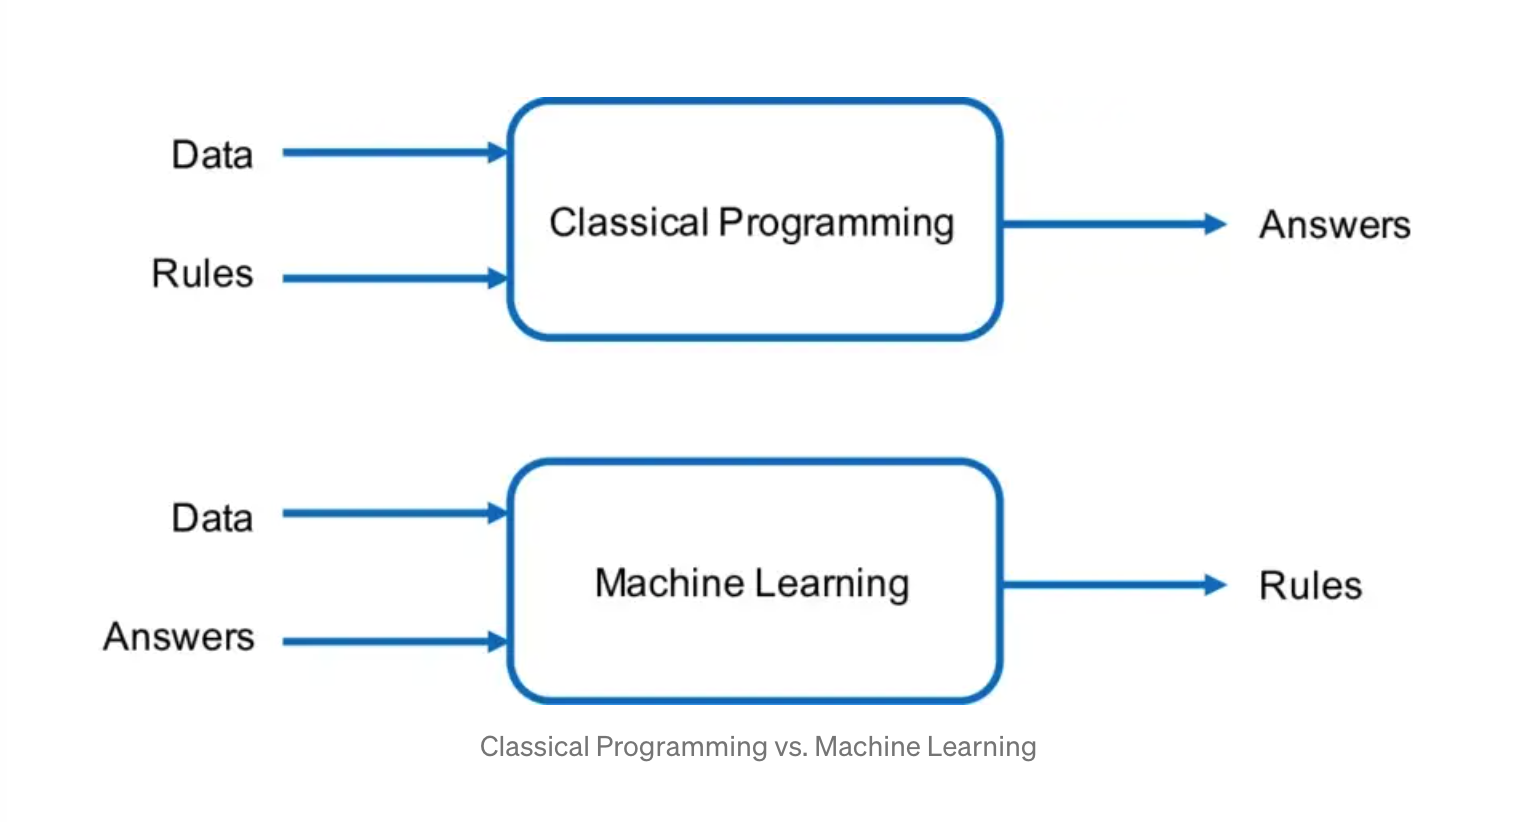
\includegraphics[width=0.8\textwidth]{../../Ressources/Figs/Fig_ProgrammingAndMLconcepts.png}
      \end{center}
   % \end{column}
  %\end{columns}
\end{frame}


\begin{frame}[allowframebreaks]{\insertsection}
\framesubtitle{Unsupervised ML}
%\begin{columns}[T] % align columns
     % \begin{column}{.5\textwidth}
%\begin{itemize}
%\end{itemize}
 %\end{column}%
    %\hfill%
    %\begin{column}{.5\textwidth}
    \begin{center}
      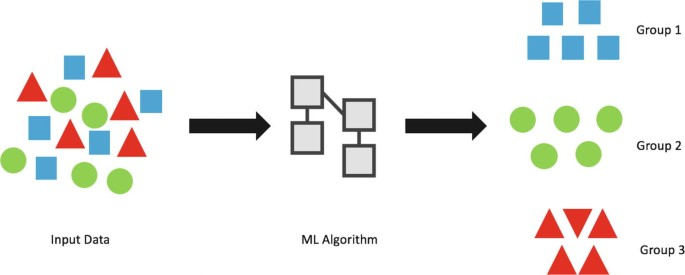
\includegraphics[width=0.9\textwidth]{../../Ressources/Figs/Fig_UnsuperviseML.jpeg}
      \end{center}
   % \end{column}
  %\end{columns}
\end{frame}

\begin{frame}[allowframebreaks]{\insertsection}
\framesubtitle{AI,  ML, Deep Learning}
%\begin{columns}[T] % align columns
     % \begin{column}{.5\textwidth}
%\begin{itemize}
%\end{itemize}
 %\end{column}%
    %\hfill%
    %\begin{column}{.5\textwidth}
    \begin{center}
     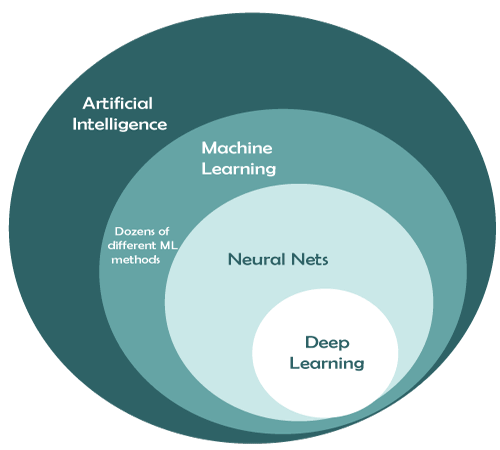
\includegraphics[width=0.5\textwidth]{../../Ressources/Figs/Fig-deep-learning-vs-machine-learning-vs-artificial-intelligence1.png}
    \end{center}
     
   % \end{column}
  %\end{columns}
\end{frame}

\begin{frame}
[allowframebreaks]{Why now?}
\begin{itemize}
\item Many of the ideas of machine learning (e.g., basic neural network by \citep{mcculloch43a}, and
perceptron by \citep{Rosenblatt1958ThePA}) are decades old.
\item Previous waves of excitement followed by backlashes.
\item Four forces behind the revival;
\item Big data.
\item Long tails.
\item Cheap computational power.
\item Algorithmic advances.
\item Likely that these four forces will become stronger over time.
\item Exponential growth in industry,
\begin{enumerate}[$\cdot$]
  \item $\Rightarrow$ plenty of libraries for Python, R, and other languages
\end{enumerate}
\end{itemize}
\end{frame}

\begin{frame}[allowframebreaks]{Popular Languages(2018)}
  \begin{columns}[T] % align columns
       \begin{column}{0.5\textwidth}
       \begin{center}
   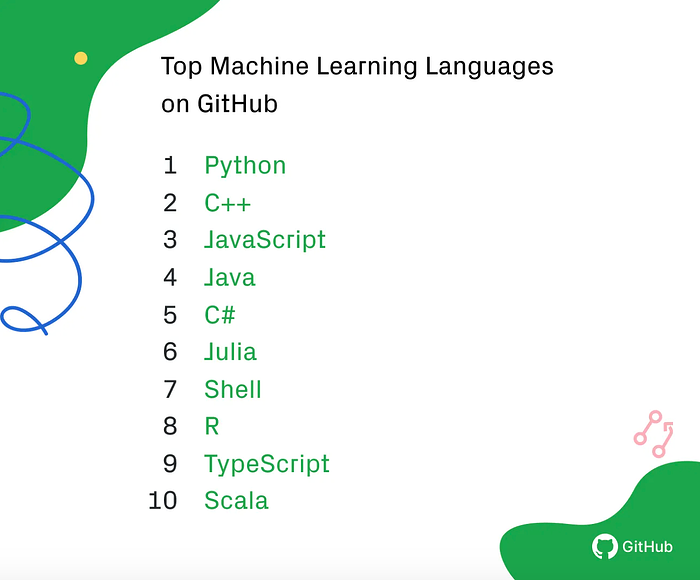
\includegraphics[width=0.6\textwidth]{../../Ressources/Figs/Fig_MostPopular2018.png}
    \end{center}
   \end{column}%
   \hfill%
   \begin{column}{0.6\textwidth}
       \begin{center}
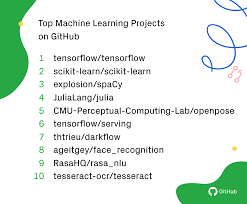
\includegraphics[width=0.5\textwidth]{../../Ressources/Figs/Fig_ProjectsGit2018.png}
 \end{center}
   \end{column}
 \end{columns}
\end{frame}

\begin{frame}[allowframebreaks]{Some DL libraries}
\begin{columns}[T] % align columns
     \begin{column}{.5\textwidth}
     \begin{center}
 
\includegraphics[width=0.4\textwidth]{../../Ressources/Figs/Fig_TensorFlowLogo.png}\\
  
\includegraphics[width=0.4\textwidth]{../../Ressources/Figs/Fig_PytorchLogo.jpeg}\\
  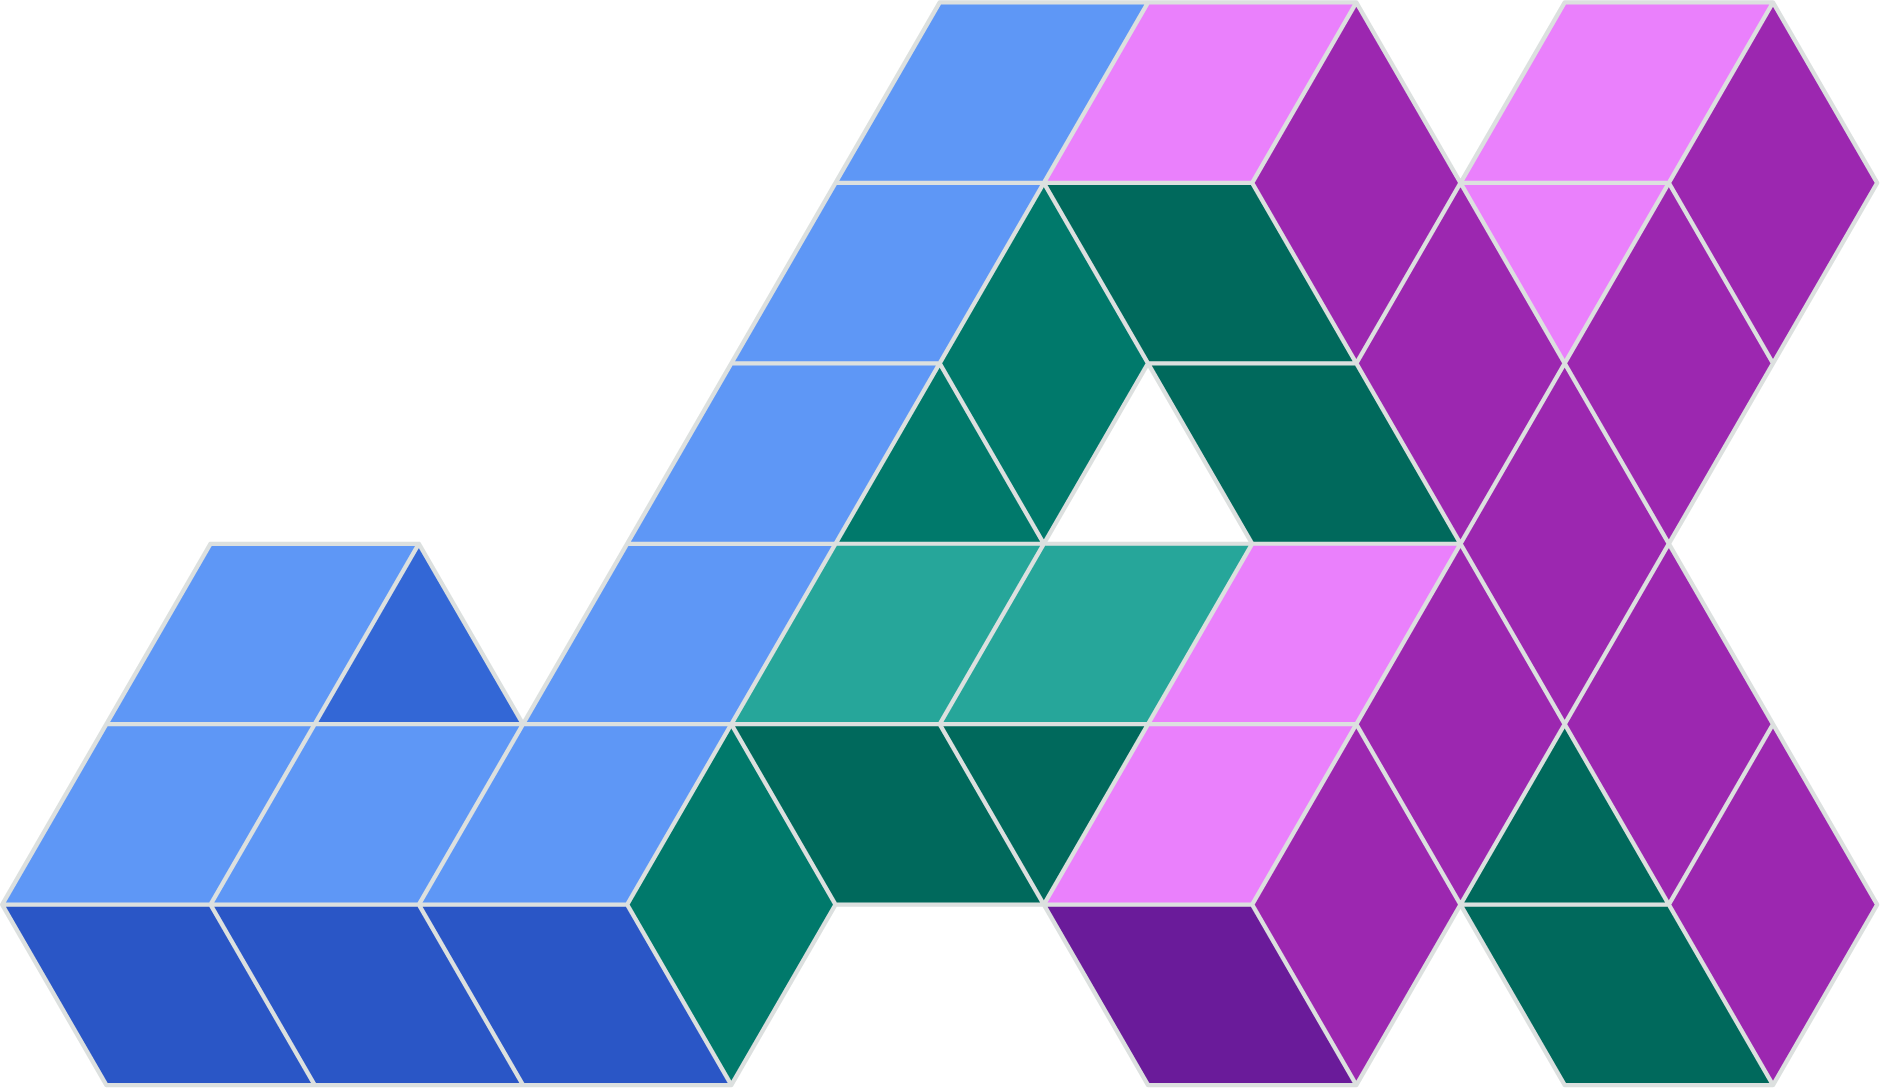
\includegraphics[width=0.4\textwidth]{../../Ressources/Figs/Fig_JaxLogo.png}
  \end{center}
 \end{column}%

    \hfill%
    \begin{column}{.5\textwidth}
        \begin{center}
 
\includegraphics[width=0.4\textwidth]{../../Ressources/Figs/Fig_FluxLogo.png}\\
  
\includegraphics[width=0.4\textwidth]{../../Ressources/Figs/Fig_CaffeLogo.jpeg}\\
  
\includegraphics[width=0.4\textwidth]{../../Ressources/Figs/Fig_CNTKLogo.png}
  \end{center}
    \end{column}
  \end{columns}
\end{frame}

\begin{frame}
[allowframebreaks]{ML in economics(some examples)}

\begin{itemize}
\item "Classical" ML:
\begin{enumerate}[$\cdot$]
\item Applied Micro / Microeconometrics(mostly for policy evaluation): \cite{MullainathanSpiessJEP2017},  \cite{AtheyImbensARE2019}, \cite{GentzkowEtalEcta2019}, \ldots 
\item Theoretical econometrics: there are many papers working on good inference practices for method using ML tools, e.g., \cite{ChernozhukovEtalAER2017}, this is an active area of research.
\item Macro : \cite{CoulombeEtalJAE2022}, \ldots 
\end{enumerate}
\item DL:
 \begin{enumerate}[$\cdot$]
 \item New solution methods for economic models: \cite{AzinovicEtalIER2022}, \ldots
\item Alternative to older bounded rationality models: reinforcement learning(e.g., \citep{FinanPouzoArxiv2021}),\ldots
\item Alternative empirical models for micro policy evaluation(aka., Treatment Effects): \cite{ChernozhukovEtalArxiv2021}, \cite{HartfordEtalProced2017}, \cite{FarreletalECTA16901}, \ldots
\end{enumerate}
\end{itemize}
\end{frame}

\section{Formal introduction and general ideas}
\frame{\sectionpage}
\begin{frame}[allowframebreaks]{The problem}
  \begin{quote}
    All exact science is dominated by the idea of approximation,
  \end{quote}
  Betrand Russell.
\begin{itemize}
\item Let us suppose we want to approximate (“learn”) an unknown function
\begin{align*}
y &= f (\boldx)
\end{align*}
where $y$ is a scalar and $\boldx \coloneqq (x_0 = 1, x_1, x_2, ..., x_p)^\top$ a vector (why a constant?).
\item We care about the case when$ p$ is large (possibly in the thousands!).
\item Easy to extend to the case where y is a vector (e.g., a probability distribution), but notation becomes
cumbersome.
\item In economics, $f (\boldx)$ can be a value function, a policy function, a pricing kernel, a conditional
expectation(e.g., a regression function), a classifier, \ldots
\end{itemize}

\end{frame}
\begin{frame}[allowframebreaks]{Neural network}
\begin{itemize}
\item A neural network is an approximation to $ f(\cdot)$ of the form:
\begin{align*}
y &\approx g^{NN}(\boldx; \boldtheta) = \theta_0 + \sum_{j=1}^k\theta_j\phi(z_j),
\end{align*}
where $\phi(\cdot)$ is an \textbf{activation function} and:
\begin{align*}
z_j &= \sum_{l=0}^p \theta_{l, j}x_l.
\end{align*}
\item The $x_l$'s  are known as the features of the data, which belong to a feature space $\mathcal{X}$ .
\item The $\phi(z_j)$’s are known as the representation of the data.
\item $k$ is known as the width of the model (wide vs. thin networks).
\item “Training” the network: selecting $\boldtheta$ such that $g^{NN}(\boldx; \boldtheta)$ is as close to $f (\boldx) $ as possible given some
relevant metric (e.g., the $\mathcal{L}^2$ norm).

\framebreak

\item \textbf{Flow representation:}

\begin{center}
 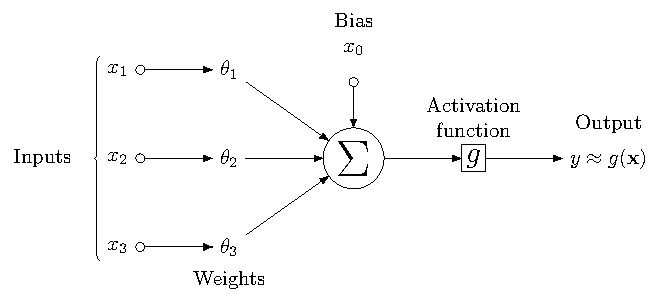
\includegraphics[width=0.8\textwidth]{../../Ressources/Figs/Fig_multilayerNet_3.pdf}\\
\end{center}
\end{itemize}

\end{frame}

\begin{frame}[allowframebreaks]{Comparison with other approximations}
\begin{itemize}
\item Compare:
\begin{align*}
  y &\approx g^{NN}(\boldx; \boldtheta) = \theta_0 + \sum_{j=1}^k\theta_j\phi\left(\sum_{l=0}^p \theta_{l, j}x_l\right),
\end{align*}
with a standard projection:
\begin{align*}
  y &\approx g^{CP}(\boldx; \boldtheta)=  \theta_0 + \sum_{j = 1}^k\theta_j\phi_j(\boldx),
\end{align*}
where  $\phi_j(\cdot)$ is, for example, a Chebyshev polynomial.
\item Note:
\begin{enumerate}[$\cdot$]
  \item We exchange the rich parameterization of coefficients for the parsimony of basis functions.
  \item In a next course, I will explain why this is often a good idea. Suffice it to say now that evaluating a neural network is straightforward.
  \item How we determine the coefficients is also different, but this is less important.
\end{enumerate}
\end{itemize}
\end{frame}


\begin{frame}[allowframebreaks]{Deep learning}
  \begin{itemize}
\item A deep learning (neural) network is a \textbf{multilayer} composition of $M > 1$ neural networks:
\begin{align*}
  &z_j^0 = \theta_{0, j}^0 + \sum_{l=1}^p\theta_{l, j}^0 x_l,\\
  \text{and}&\\
  &z_j^1 = \theta_{0, j}^1 + \sum_{j=1}^{k_1}\theta_j^1\phi^1(z_j^0)\\
  &\vdots\\
  & y \approx g^{DL}(\boldx; \boldtheta) = \theta_0^M + \sum_{j = 1}^{k_M}\theta_j^M\phi^M(z_j^{M-1}),
  \end{align*}
  where the $k_1$, $k_2$,\ldots,  and $\phi^1(\cdot)$, $\phi_2(\cdot)$, \ldots
   are possibly different across each layer of the network.
  

  \framebreak 
  \item \textbf{Flow representation:}
  \begin{center}
    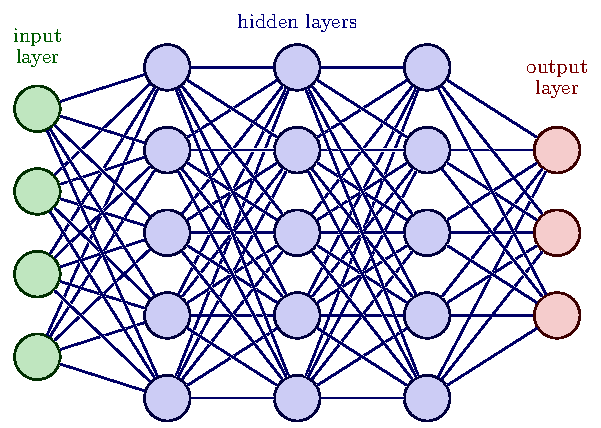
\includegraphics[width=0.6\textwidth]{../../Ressources/Figs/Fig_multilayerNet_2.pdf}\\
   \end{center}

   \framebreak

   \item $M$ is known as the depth of the network (deep vs. shallow networks). 
   The case $M = 1$ is the neural network we saw before.
\item From now on, we will refer to neural networks as including both single and multilayer networks.
\item As before, we select $\boldtheta$ such that $g^{DL}(\boldx; \boldtheta)$
 approximates a target function $f(\boldx)$ as closely as possible under some relevant metric.
\item We can also add multidimensional outputs.
\item Or even to produce a probability distribution as output, 
for example, using a \textbf{softmax layer}:
\begin{align*}
y_j &= \frac{exp(z_j^{M-1})}{\sum_{j=1}^k \exp(z_j^{M-1})}.
\end{align*}
\item All other aspects (selecting $\phi(\cdot)$, $M$, $k$, \ldots) 
are known as the network architecture. We will discuss extensively 
further in the course how to determine them.
\end{itemize}
\end{frame}

\begin{frame}[allowframebreaks]{Why do neural networks “work”?}
\begin{itemize}
  \item Neural networks consist entirely of chains of tensor operations:
   we take $\boldx$, we perform affine transformations, and apply an activation function.
\item Thus, these tensor operations are geometric transformations of $\boldx$.
\item In other words: a neural network is a complex geometric transformation 
in a high-dimensional space.
\item Deep neural networks look for convenient geometrical representations of high-dimensional manifolds.
\item The success of any functional approximation problem is to search for the 
right geometric space in which to perform it, not to search for a “better” basis function.

\framebreak 
\begin{center}
  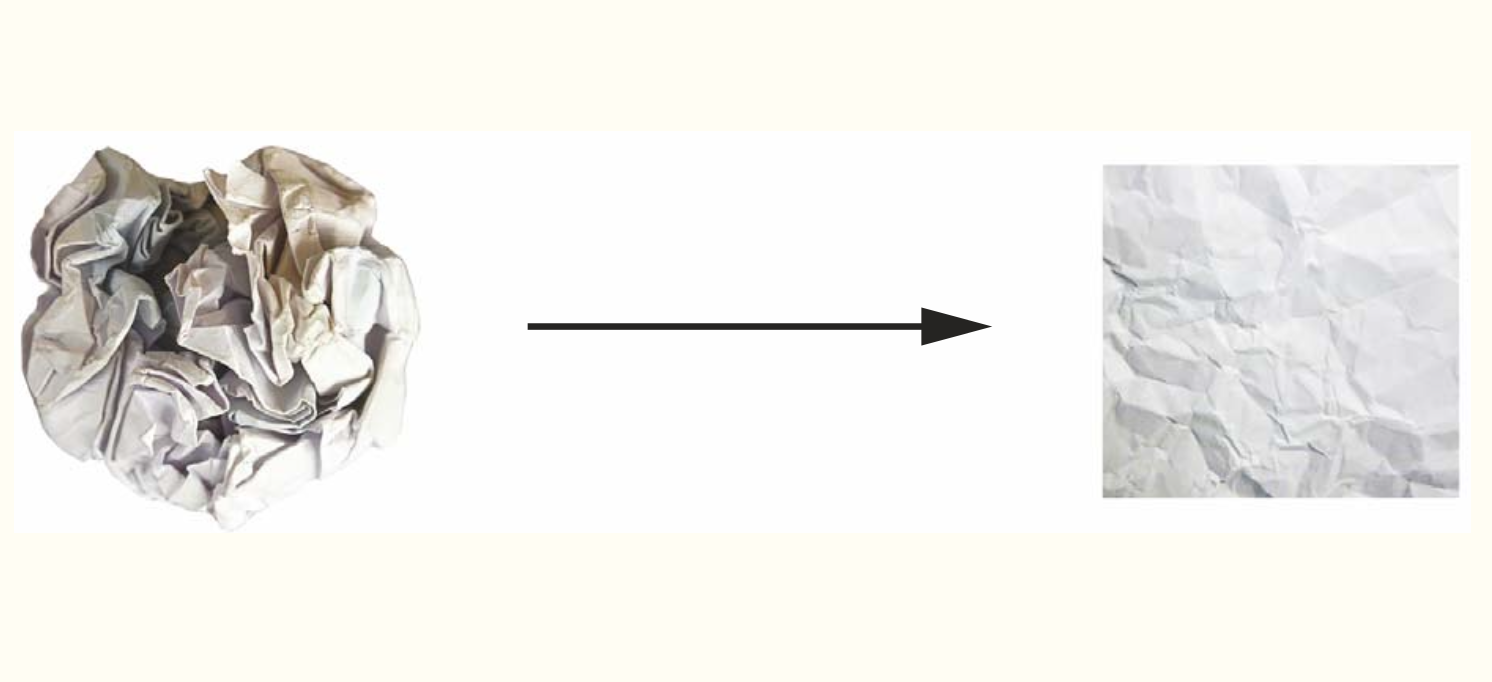
\includegraphics[width=0.8\textwidth]{../../Ressources/Figs/Fig_NeuralNetsWhyTheyWork.png}\\
 \end{center}

\end{itemize}
\end{frame}

\begin{frame}[allowframebreaks]{Why do deep neural networks “work” better?}
\begin{itemize}
  \item Why do we want to introduce hidden layers?
  \begin{enumerate}
  \item It works! Evolution of ImageNet winners.
  \item The number of representations increases
   exponentially with the number of hidden layers while
    computational cost grows linearly.
  \item Intuition: hidden layers induce highly nonlinear 
  behavior in the joint creation of representations without 
  the need to have domain knowledge (used, in other algorithms, 
  in some form of greedy pre-processing).
  \end{enumerate}

  \framebreak 

\begin{center}
  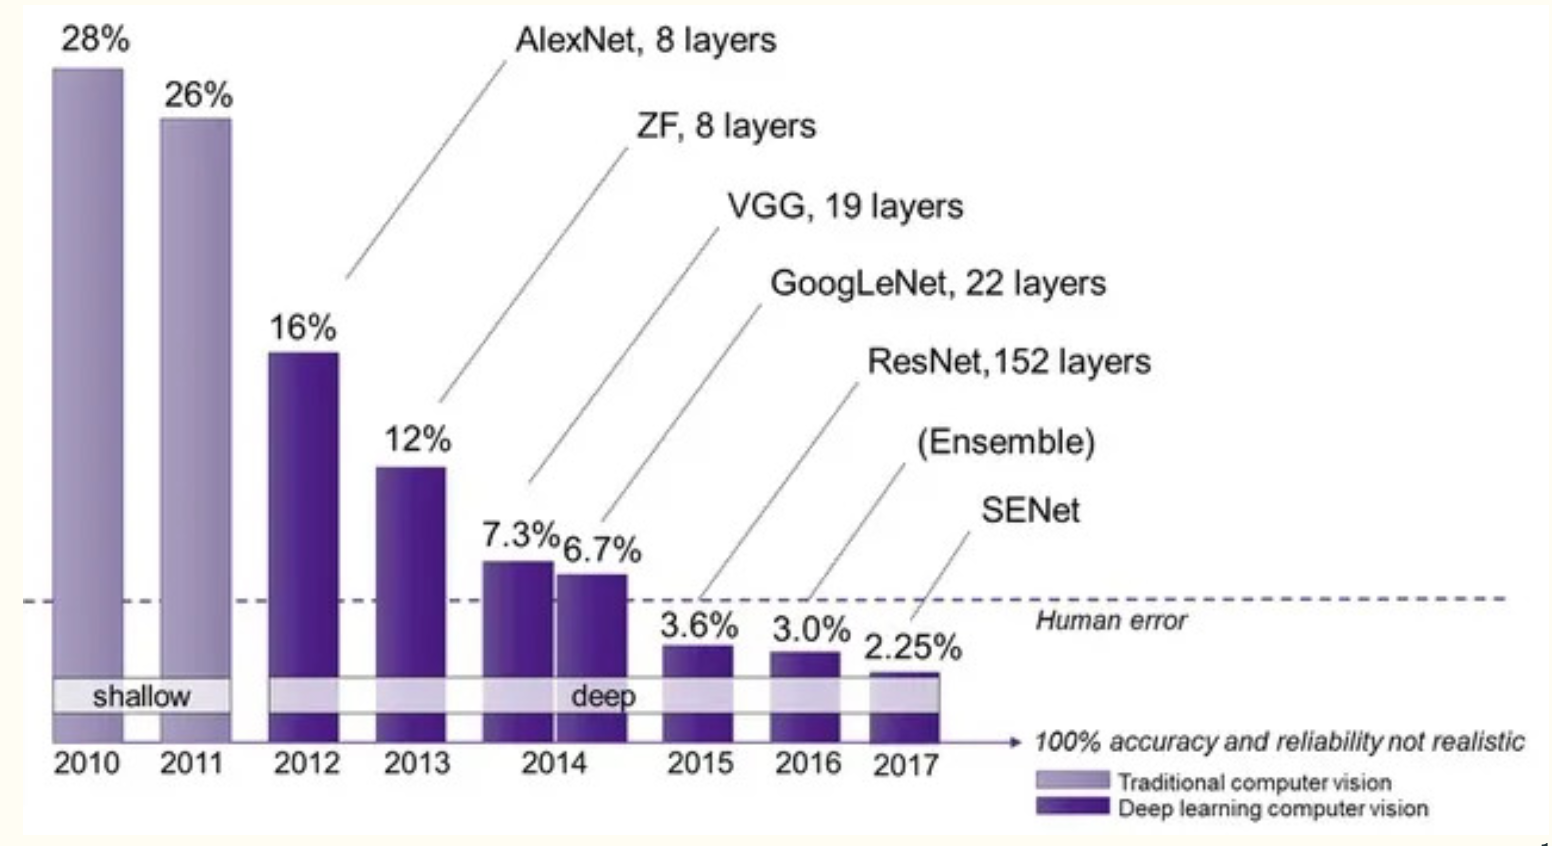
\includegraphics[width=0.8\textwidth]{../../Ressources/Figs/Fig_AccuracyNetsVision.png}\\
 \end{center}


\end{itemize}
\end{frame}


\begin{frame}[allowframebreaks]{Some consequences}
\begin{itemize}
  
  \item Because of the previous arguments, neural networks 
  can efficiently approximate extremely complex functions.
  \item In particular, under certain (relatively weak) conditions:
  \begin{enumerate}
  \item Neural networks are universal approximators.
  \item Neural networks break the “curse of dimensionality.”
  \end{enumerate}
  \item Furthermore, neural networks are easy to code, stable, 
  and scalable for multiprocessing (neural networks are built around tensors).
  \item The richness of an ecosystem is key for its long-run success.

\end{itemize}

\end{frame}


\section{Introduction to deep learning for econometrics}
\frame{\sectionpage}
\begin{frame}[allowframebreaks]{Takeaways}
\begin{itemize}
\item Deep learning is regression with complicated functional forms.
\item Design considerations in feedforward networks include depth, width, and the
connections between layers.
\item Optimization is difficult in deep learning because of
\begin{enumerate}
\item lots of data
\item  and even more parameters
\item in a highly non-linear model.
\end{enumerate}
\item $\Rightarrow$  Specially developed optimization methods.
\item Cross-validation for penalization is computationally costly, as well.
\item A popular alternative is sample-splitting and early stopping.
\end{itemize}
\end{frame}

\section{Setup: what are neural nets?}
\frame{\sectionpage}
\begin{frame}[allowframebreaks]{Deep Neural Nets}
  \framesubtitle{Setup}
%\underline{\textbf{Setup}}
    \begin{itemize}
    \item  Deep learning is (regularized) maximum likelihood, for regressions with
complicated functional forms.
\item We want, for instance, to find $\boldtheta$ to minimize
\begin{align*}
\Exp\left[((Y - f(X, \boldtheta))^2\right],
\end{align*}
for continuous outcomes $Y$, or to maximize
\begin{align*}
\Exp\left[\sum_{y}\Ind(Y = y)\cdot\log\left(f(X, \boldtheta)\right)^2\right]
\end{align*}
for discrete outcomes $Y$.
    \end{itemize}
\end{frame}

\begin{frame}[allowframebreaks]{What’s deep about that?}
\framesubtitle{Feedforward nets}
\begin{itemize}
  \item Functions $f$ used for deep (feedforward) nets can be written as
  \begin{align*}
  f(x,\boldtheta) &= f^k\left(f^{k-1}
  \left(\ldots f^1(\boldx, \boldtheta^1), \boldtheta^2\right),\ldots, \boldtheta^k\right).
  \end{align*}
  \item Biological analogy:
  \begin{enumerate}[$\cdot$]
  \item Each value of a component of $f$
  j corresponds to the “activation” of a “neuron.”
  \item Each $f^j$ corresponds to a layer of the net: Many layers $\Rightarrow$ “deep” neural net.
  \item The layer-structure and the parameters $\boldtheta$ determine how these neurons are
  connected.
  \end{enumerate}
  \item Inspired by biology, but practice moved away from biological models.
  \item Best to think of as a class of nonlinear functions for regression.
\end{itemize}
\end{frame}

\begin{frame}[allowframebreaks]{So what’s new?}
\begin{itemize}
\item Very non-linear functional forms f. Crucial when
\begin{enumerate}[$\cdot$]
\item mapping pixel colors into an answer to “Is this a cat?,”
\item or when mapping English sentences to Mandarin sentences.
\item Probably less relevant when running Mincer-regressions.
\end{enumerate}
\item Often more parameters than observations.
\begin{enumerate}[$\cdot$]
  \item Not identified in the usual sense.
But we care about predictions, not parameters.
\item Overparametrization helps optimization:
Less likely to get stuck in local minima.
\end{enumerate}
\item Lots of computational challenges.
\begin{enumerate}
\item Calculating gradients:
Backpropagation, stochastic gradient descent.
\item Searching for optima.
\item Tuning: Penalization, early stopping.
\end{enumerate}
\end{itemize}
\end{frame}
\section{Network design}
\frame{\sectionpage}
\begin{frame}[allowframebreaks]{\insertsection}
  \framesubtitle{Activation functions}
    \begin{columns}[T] % align columns
      \begin{column}{.5\textwidth}
        \begin{itemize}
        \item Basic unit of a net: a neuron $i$ in layer $j$.
        \item Receives input vector $x_j^i$(output of other neurons).
        \item Produces output $g(x^j_i, \boldtheta^j_i + \boldeta_i^j)$.
        \item Activation function $g(\cdot)$:
         \begin{enumerate}[$\cdot$]
          \item Older nets: Sigmoid function
          (biologically inspired).
          \item Modern nets: “Rectified linear
          units:” $g\left(\max(0, z)\right)$: 
          More convenient for getting
          gradients.
          \end{enumerate}
        \end{itemize}
      \end{column}%
    \hfill%
    \begin{column}{.5\textwidth}
      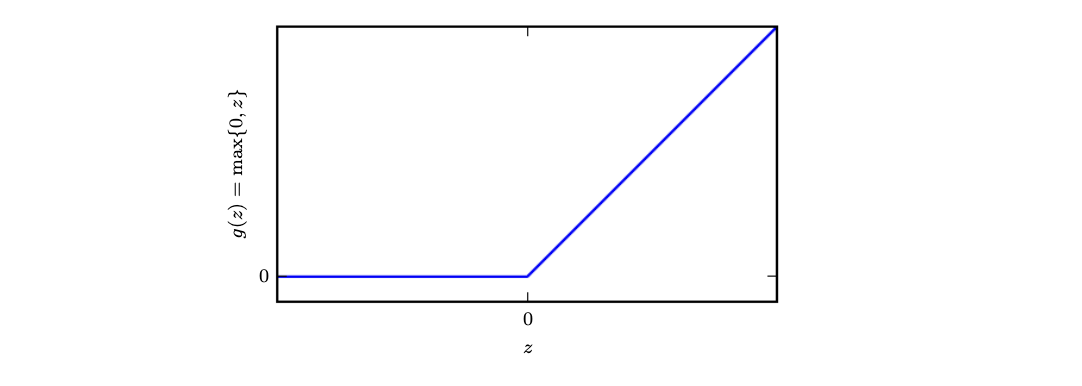
\includegraphics[width=9cm,height=5cm]{../../Ressources/Figs/Fig_DPbook_Goodfellow_et_al_activationFunction_chapt6.png}
    \end{column}
  \end{columns}
\end{frame}

\begin{frame}{\insertsection}
  \framesubtitle{Architecture}
  \begin{itemize}
\item These neurons are connected, usually structured by layers.\\
Number of layers: Depth. Number of neurons in a layer: Width.
\item Input layer: Regressors.
\item Output layer: Outcome variables.
\item A typical example:
\begin{figure}
  \begin{center}
      \scalebox{0.7}{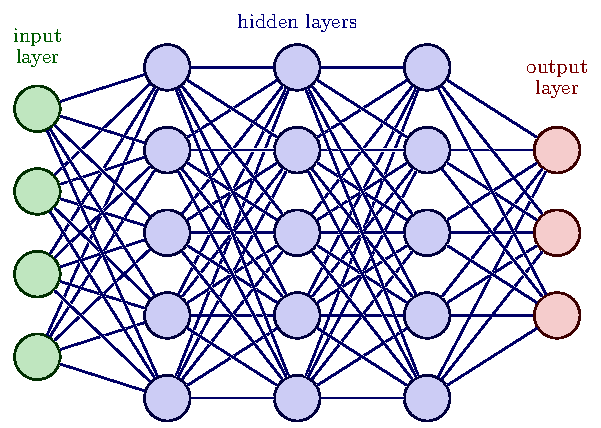
\includegraphics{../../Ressources/Figs/Fig_multilayerNet_2.pdf}}
   \vspace{1em}
  \end{center}
\end{figure}
  \end{itemize}
\end{frame}

  \begin{frame}{\insertsection}
    \framesubtitle{Architecture}
  \begin{itemize}
    \item Suppose each layer is fully connected to the next, and we are using RELU
    activation functions.
    \item Then we can write in matrix notation (using componentwise $\max$):
    \begin{align*}
      \boldx^j &= f^j\left(\boldx^{j-1}, \boldtheta^j\right) = \max\left(0, \boldx^{j-1}\cdot\boldtheta^j+\boldeta_j\right),
    \end{align*}
  \item Matrix $\boldtheta^j$:
  \begin{enumerate}[$\cdot$]
  \item Number of rows: Width of layer $j-1$.
  \item Number of columns: Width of layer $j$.
  \end{enumerate}
  \item Vector $\boldx^j$:
  \begin{enumerate}[$\cdot$]
  \item Number of entries: Width of layer $j$.
  \end{enumerate}
  \item Vector $\eta_j$:
  \begin{enumerate}[$\cdot$]
  \item Number of entries: Width of layer $j$.
  \item Intercepts. Confusingly called “bias” in machine learning.
\end{enumerate}
  \end{itemize}
\end{frame}

\begin{frame}[allowframebreaks]{\insertsection}
\framesubtitle{Output layer}
\begin{itemize}
\item Last layer is special: Maps into predictions.
\item Leading cases:
\begin{enumerate}
\item Linear predictions for continuous outcome variables,
\begin{align*}
  f^k(\boldx^{k-1},\boldtheta^k) &=\boldx^{k-1}\cdot\boldtheta^k.
\end{align*}
\item Multinomial logit (aka “softmax”) predictions for discrete variables,
\begin{align*}
f^{k, y_j}(\boldx^{k-1},\boldtheta^k)  &=\frac{\exp(\boldx^{k-1}_j\cdot\boldtheta^k_j)}
{\sum_{j^\prime} \exp(\boldx^{k-1}_{j^\prime}\cdot\boldtheta^k_{j^\prime})}
\end{align*}
\end{enumerate}
\item Network with only output layer: Just run OLS / multinomial logit.
\end{itemize}
\end{frame}

\section{Backpropagation}
\frame{\sectionpage}
\begin{frame}[allowframebreaks]{\insertsection}
\framesubtitle{The chain rule}
\begin{itemize}
\item In order to maximize the (penalized) likelihood, we need its gradient.
\item Recall that 
 \begin{align*}
  f(x,\boldtheta) &= f^k\left(f^{k-1}
  \left(\ldots f^1(\boldx, \boldtheta^1), \boldtheta^2\right),\ldots, \boldtheta^k\right).
  \end{align*}
  \item By the chain rule:
  \begin{align*}
  \frac{\partial f(\boldx, \boldtheta)}{\partial \boldtheta_i^j} &=\left(\prod_{j^\prime = j+1}^k \frac{\partial f^{j^\prime}(\boldx^{j^\prime}, \boldtheta^j)}
  {\partial \boldx^{j^\prime - 1} }\right)\cdot\frac{\partial f^j(\boldx^{j-1}, \boldtheta^j)}{\partial \boldtheta_i^j}.
  \end{align*}
  \item A lot of the same terms show up in derivatives w.r.t different $\boldtheta^j_i$:
\begin{enumerate}[$\cdot$]
\item $\boldx^{j^\prime}_i$(values of layer $j^\prime$).
\item $\frac{\partial f^{j^\prime}(\boldx^{j^\prime}, \boldtheta^j)}{\partial \boldx^{j^\prime - 1} }$(intermediate layer derivatives w.r.t. $\boldx^{j^\prime-1}$).

\end{enumerate}
\end{itemize}

\framebreak

\begin{itemize}
\item Denote $\boldz^j = \boldx^{j-1}\boldtheta^j+\eta^j$. Recall $\boldx^j= \max(0,\boldz^j)$.
\item Note $\frac{\partial \boldx^j}{\partial \boldz^j} = \Ind\left(\boldz^j \geq 0 \right)$(componentwise), and $\frac{\partial \boldz^j}{\partial\boldtheta^j} = \boldx^{j-1}$.
\item First, \textbf{forward propagation}:
Calculate all the $\boldz^j$ and $\boldx^j$
starting at $ j = 1$
\item Then \textbf{backpropagation}:
Iterate backward, starting at $ j = k$;
\begin{enumerate}
\item Calculate and store
\begin{align*}
\frac{\partial f(\boldx, \boldtheta)}{\partial \boldx^{j-1}}&=\frac{\partial f(\boldx, \boldtheta)}{\partial\boldx^j}\cdot\Ind(\boldz^j\geq 0)\boldtheta^{j^\prime}.
\end{align*}
\item Calculate
\begin{align*}
\frac{\partial f(\boldx, \boldtheta)}{\partial \boldtheta^j}&=\frac{\partial f(\boldx, \boldtheta)}{\partial \boldx^j}\cdot\Ind(\boldz^j\geq 0)\boldx^{j-1}.
\end{align*}
\end{enumerate}
\end{itemize}
\end{frame}

\begin{frame}[allowframebreaks]{\insertsection}
\framesubtitle{Advantages}
\begin{itemize}
\item Backpropagation improves efficiency by \textbf{storing} intermediate derivatives,
\textbf{rather than recomputing} them.
\item Number of computations grows only linearly in number of parameters.
\item The algorithm is easily generalized to more complicated network architectures
and activation functions.
\item Parallelizable across observations in the data (one gradient for each
observation!).

\end{itemize}
\end{frame}
\begin{frame}[allowframebreaks]{References}
\bibliographystyle{jpe}
\bibliography{../../Biblio}
\end{frame}

\end{document}
